\documentclass[journal]{IEEEtran}
\IEEEoverridecommandlockouts

\usepackage{cite}
\usepackage{amsmath,amssymb,amsfonts}
\usepackage{graphicx}
\usepackage{subcaption}
\usepackage{booktabs}
\usepackage{multirow}
\usepackage{textcomp}
\usepackage{xcolor}
\usepackage{tikz}
\usetikzlibrary{arrows.meta, positioning, fit, backgrounds, shapes.symbols, calc}
\usepackage{algorithm}
\usepackage{algorithmicx}
\usepackage{algpseudocode}
\newtheorem{definition}{Definition}
\newtheorem{remark}{Remark}

% --- float placement relaxation (layout only) ---
\renewcommand{\topfraction}{0.92}
\renewcommand{\bottomfraction}{0.85}
\renewcommand{\textfraction}{0.06}
\renewcommand{\floatpagefraction}{0.75}
\renewcommand{\dbltopfraction}{0.92}
\renewcommand{\dblfloatpagefraction}{0.75}
\setcounter{topnumber}{3}
\setcounter{bottomnumber}{2}
\setcounter{totalnumber}{4}
\setcounter{dbltopnumber}{3}
% --- vertical spacing tightening (layout only, no content change) ---
\setlength{\textfloatsep}{9pt plus 2pt minus 2pt}
\setlength{\dbltextfloatsep}{10pt plus 2pt minus 2pt}
\setlength{\floatsep}{8pt plus 2pt minus 2pt}
\setlength{\intextsep}{8pt plus 2pt minus 2pt}
\setlength{\abovedisplayskip}{5pt plus 2pt minus 2pt}
\setlength{\belowdisplayskip}{5pt plus 2pt minus 2pt}
\setlength{\abovedisplayshortskip}{3pt plus 2pt}
\setlength{\belowdisplayshortskip}{3pt plus 2pt}
% --- float-column glue: pin floats to top, small fixed gap between ---
\makeatletter
\setlength{\@fptop}{0pt}
\setlength{\@fpsep}{6pt plus 2pt}
\setlength{\@fpbot}{0pt plus 1fil}
\makeatother

\def\BibTeX{{\rm B\kern-.05em{\sc i\kern-.025em b}\kern-.08em
    T\kern-.1667em\lower.7ex\hbox{E}\kern-.125emX}}
\begin{document}

\title{SPARC: Semi-Markov Per-User Charging Chains for Synthetic EV Charging-Session Data Generation}
%Muhammad~Amir~Hamza,~Benoit~Boulet,~and~Di~Wu%
\author{
% \thanks{This research is funded by Flo.}%
\thanks{M.~A.~Hamza and B.~Boulet are with the Department of Electrical and Computer Engineering, McGill University, Montreal, QC, Canada (e-mail: muhammad.hamza@mail.mcgill.ca; benoit.boulet@mcgill.ca).}%
\thanks{D.~Wu is with the Department of Mechanical, Industrial \& Aerospace Engineering, Concordia University, Montreal, QC, Canada (e-mail: di.wu@concordia.ca).}}

\markboth{IEEE Transactions on Smart Grid,~Vol.~XX, No.~XX, 2026}%
{Hamza \MakeLowercase{\textit{et al.}}: SPARC: Per-User Semi-Markov EV Charging Session Generation}

\maketitle

\begin{abstract}
Session-level electric-vehicle (EV) charging data is essential for grid-impact studies, smart-charging design, and simulators, yet remains scarce due to privacy concerns and commercial competitiveness. Existing synthetic generators pool all users into one distribution or require large training sets, discarding individual recurring behavior. We present SPARC, a per-user semi-Markov paradigm that captures each user's recurring charging routine and generates statistically faithful, temporally consistent, and flexible synthetic sessions. A session-as-state encoding records habitual patterns, and per-bin distributions selected by the Bayesian information criterion (BIC) model arrival time, plug-in duration, energy, and idle gap. For users with less data, a three-level fallback stabilizes the fits, and a convolution diagnostic adds a copula correction only where duration--gap dependence appears. A two-stream weekday/weekend simulator replays each user over arbitrary horizons, and a four-level protocol validates from marginals to aggregate load. Across four cohorts spanning residential, workplace, and commercial charging, per-driver and per-station, SPARC validates from tens of sessions per user; against copula, deep-generative, and parametric baselines it matches aggregate marginal fidelity while uniquely preserving the between-user heterogeneity they collapse. SPARC thus provides realistic, controllable charging populations for distribution-grid studies, simulators and digital twins, and the training and benchmarking of learning-based charging strategies.
\end{abstract}

\begin{IEEEkeywords}
Electric Vehicle Charging, Synthetic Data Generation, Semi-Markov Chains, Charging Behavior Modeling, Load Modeling, Smart Charging, Generative Models
\end{IEEEkeywords}

\section{Introduction}
\label{sec:introduction}


EV charging is fast becoming one of the largest new loads on distribution grids~\cite{li2024impact}. It is also concentrated: home charging alone accounts for roughly 64\% of U.S. charging activity~\cite{nrel2023}, and home plus workplace deliver 80--86\% of all charging energy~\cite{iea2024, icct2024}. In both settings, most sessions come from recurring users with fixed routines: residents returning home, commuters arriving at work. When these routines coincide, they produce sharp local peaks that stress feeders and overload distribution transformers~\cite{li2024impact}. Smart-charging design~\cite{sastry2023decentralized}, infrastructure planning, demand-response evaluation, reinforcement-learning control~\cite{xing2023bilevel}, and grid simulators and digital twins~\cite{yu2024digital} all need session-level data: individual plug-in times, durations, and energies. They also need \emph{controllable} data: populations that can be resized, recomposed, and simulated over any horizon~\cite{powell2022scalable}. Yet operators rarely release charging logs, which are privacy-sensitive and commercially sensitive~\cite{calearo2021, li2025trc}.

% Auto-generated from figures/sparc_framework.tex (standalone). Do not hand-edit;
% regenerate from the standalone so the two stay in sync.
% Preamble needs: \usetikzlibrary{arrows.meta,positioning,fit,backgrounds,shapes.symbols,calc}
\begin{figure}[t]
\centering
\resizebox{0.94\columnwidth}{!}{%
\newcommand{\mchain}[3]{%
  \begin{scope}[shift={(#1,#2)}]
    \node[st,draw=#3] (ma) at (-0.36, 0.08) {};
    \node[st,draw=#3] (mb) at ( 0.28, 0.16) {};
    \node[st,draw=#3] (mc) at (-0.04,-0.30) {};
    \draw[-{Latex[length=1.4mm,width=1.2mm]},semithick,color=#3] (ma) -- (mb);
    \draw[-{Latex[length=1.4mm,width=1.2mm]},semithick,color=#3] (mb) -- (mc);
    \draw[-{Latex[length=1.4mm,width=1.2mm]},semithick,color=#3] (mc) -- (ma);
    \draw[-{Latex[length=1.4mm,width=1.2mm]},semithick,color=#3]
         (mb) to[out=55,in=115,looseness=5] (mb);
  \end{scope}}

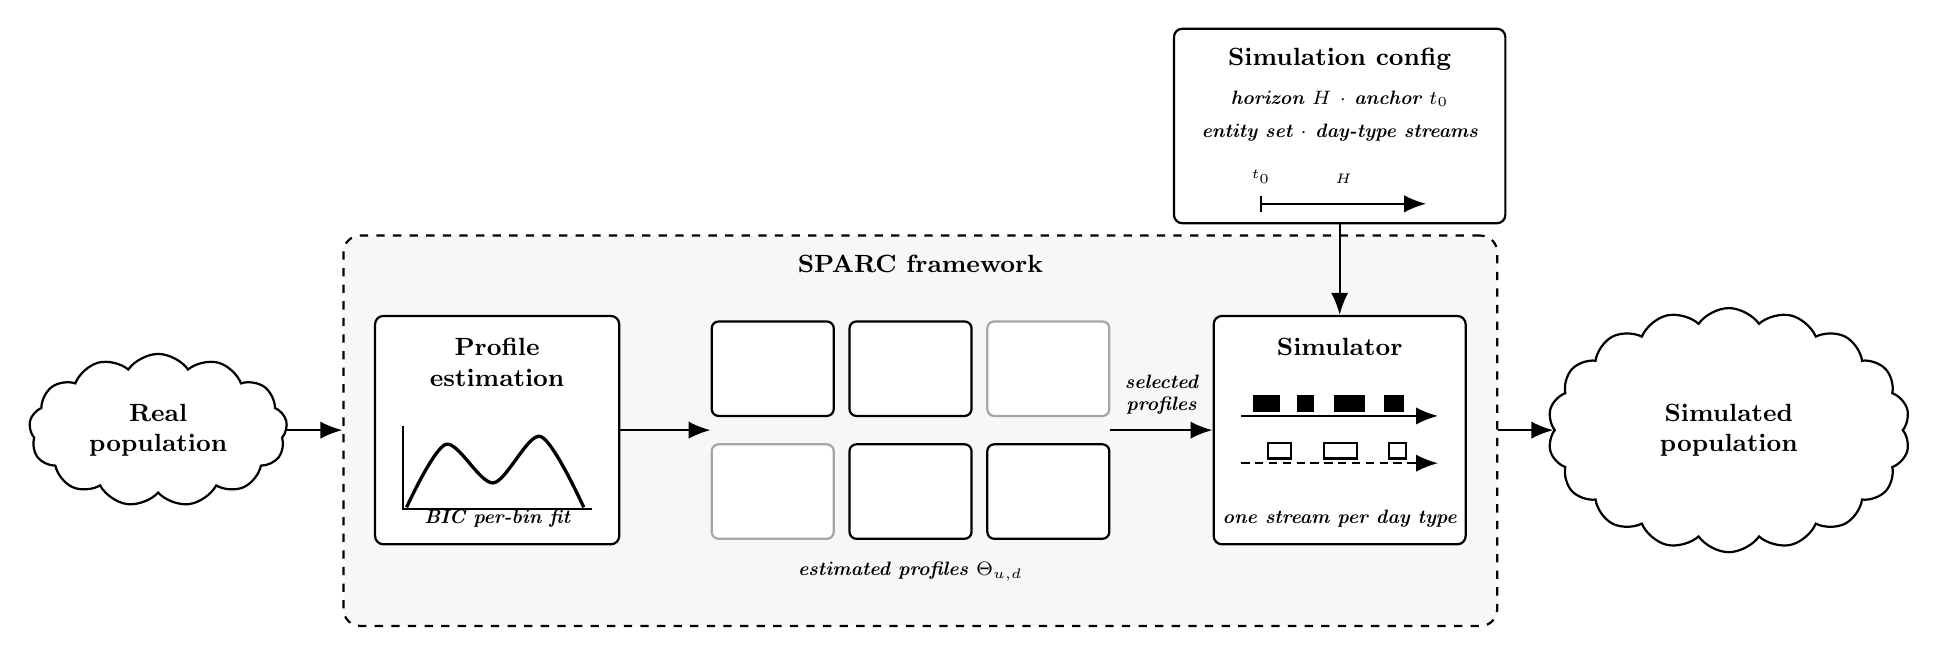
\begin{tikzpicture}[
  >={Latex[length=2.8mm,width=2.2mm]},
  arrow/.style={->, thick},
  block/.style={draw, thick, rounded corners=3pt, fill=white, align=center},
  card/.style={draw, thick, rounded corners=2.5pt, fill=white,
               minimum width=1.55cm, minimum height=1.2cm},
  gcard/.style={card, draw=black!35},
  st/.style={circle, draw, thick, fill=white, inner sep=0pt, minimum size=7pt},
  capt/.style={font=\scriptsize\itshape\bfseries, align=center},
  cloudnode/.style={cloud, draw, thick, cloud puffs=13, cloud puff arc=110,
                    aspect=2.0, align=center, font=\small\bfseries, inner ysep=1.5ex}
]

%=================== Profile estimation ===================
\node[block, minimum width=3.1cm, minimum height=2.9cm] (pe) at (4.9,0) {};
\node[anchor=north, font=\small\bfseries, align=center]
      at ([yshift=-5pt]pe.north) {Profile\\estimation};
\begin{scope}[shift={([xshift=-1.2cm,yshift=-1.0cm]pe.center)}]
  \draw[thick] (0,1.05) -- (0,0) -- (2.4,0);
  \draw[very thick] plot[smooth]
    coordinates {(0.05,0.02) (0.55,0.82) (1.15,0.33) (1.75,0.92) (2.3,0.02)};
\end{scope}
\node[capt, anchor=south] at ([yshift=3pt]pe.south) {BIC per-bin fit};

%=================== Profile bank (2 x 3 cards, small Markov chains) ===================
\node[card]  (c1) at ( 8.40, 0.78) {};
\node[card]  (c2) at (10.15, 0.78) {};
\node[gcard] (c3) at (11.90, 0.78) {};
\node[gcard] (c4) at ( 8.40,-0.78) {};
\node[card]  (c5) at (10.15,-0.78) {};
\node[card]  (c6) at (11.90,-0.78) {};

\mchain{ 8.40}{ 0.78}{black}
\mchain{10.15}{ 0.78}{black}
\mchain{11.90}{ 0.78}{black!35}
\mchain{ 8.40}{-0.78}{black!35}
\mchain{10.15}{-0.78}{black}
\mchain{11.90}{-0.78}{black}

\node[capt] at (10.15,-1.80) {estimated profiles $\Theta_{u,d}$};

%=================== Simulator (session bars on two streams) ===================
\node[block, minimum width=3.2cm, minimum height=2.9cm] (sim) at (15.6,0) {};
\node[anchor=north, font=\small\bfseries] at ([yshift=-5pt]sim.north) {Simulator};
\begin{scope}[shift={([xshift=-1.25cm]sim.center)}]
  % weekday stream: solid axis, filled session bars
  \draw[->, thick] (0,0.18) -- (2.5,0.18);
  \filldraw[fill=black, draw=black] (0.15,0.24) rectangle (0.48,0.44);
  \filldraw[fill=black, draw=black] (0.72,0.24) rectangle (0.92,0.44);
  \filldraw[fill=black, draw=black] (1.18,0.24) rectangle (1.56,0.44);
  \filldraw[fill=black, draw=black] (1.82,0.24) rectangle (2.06,0.44);
  % weekend stream: dashed axis, outlined session bars
  \draw[->, thick, dash pattern=on 3pt off 2pt] (0,-0.42) -- (2.5,-0.42);
  \filldraw[fill=white, draw=black, thick] (0.34,-0.36) rectangle (0.63,-0.16);
  \filldraw[fill=white, draw=black, thick] (1.05,-0.36) rectangle (1.47,-0.16);
  \filldraw[fill=white, draw=black, thick] (1.88,-0.36) rectangle (2.09,-0.16);
\end{scope}
\node[capt, anchor=south] at ([yshift=3pt]sim.south) {one stream per day type};

%=================== Simulation config (external, above simulator) ===================
\node[block, anchor=south, inner xsep=10pt, inner ysep=7pt]
  (cfg) at ([yshift=1.15cm]sim.north)
  {\small\bfseries Simulation config\\[2pt]
   \scriptsize\itshape\bfseries horizon $H$ $\cdot$ anchor $t_0$\\
   \scriptsize\itshape\bfseries entity set $\cdot$ day-type streams\\[12pt]
   \mbox{}};
% mini t0 -> H horizon axis in the lower part of the config box
\draw[->, thick] ([xshift=-1.00cm,yshift=0.26cm]cfg.south)
                 -- ([xshift=1.10cm,yshift=0.26cm]cfg.south);
\draw[thick] ([xshift=-1.00cm,yshift=0.16cm]cfg.south)
             -- ([xshift=-1.00cm,yshift=0.36cm]cfg.south);
\node[font=\tiny, anchor=south] at ([xshift=-1.00cm,yshift=0.40cm]cfg.south) {$t_0$};
\node[font=\tiny, anchor=south] at ([xshift= 0.05cm,yshift=0.40cm]cfg.south) {$H$};

%=================== SPARC framework frame (drawn behind) ===================
% invisible pads give the frame headroom for its title and the bottom caption
\coordinate (frametoppad) at ($(pe.north)+(0,0.62)$);
\coordinate (framebotpad) at (10.15,-2.10);
\begin{scope}[on background layer]
  \node[draw, thick, dashed, rounded corners=6pt, fill=black!3, inner sep=11pt,
        fit=(pe)(c1)(c6)(sim)(frametoppad)(framebotpad)] (frame) {};
\end{scope}
\node[anchor=north, font=\small\bfseries] at ([yshift=-4pt]frame.north)
      {SPARC framework};

%=================== Population clouds ===================
\node[cloudnode, anchor=east] (real)
      at ($(frame.west |- 0,0)+(-0.7,0)$) {Real\\population};
\node[cloudnode, anchor=west, minimum width=4.6cm, minimum height=3.1cm,
      cloud puffs=18] (simpop)
      at ($(frame.east |- 0,0)+(0.7,0)$) {Simulated\\population};

%=================== Main arrows (all on the y=0 midline) ===================
\draw[arrow] (real.east)          -- (frame.west |- 0,0);
\draw[arrow] (pe.east)            -- (c1.west |- 0,0);
\draw[arrow] (c3.east |- 0,0)     -- (sim.west);
\draw[arrow] (frame.east |- 0,0)  -- (simpop.west);
\draw[arrow] (cfg.south)          -- (sim.north);
\node[capt] at ($(c3.east |- 0,0)!0.5!(sim.west)+(0,0.45)$)
      {selected\\profiles};

\end{tikzpicture}
}
\caption{SPARC learns per-entity behaviour as semi-Markov profiles and replays them with a configurable simulator to generate a synthetic charging population.}
\label{fig:framework}
\end{figure}


\begin{table*}[t]
\centering
\caption{Session-level generators vs.\ properties P1--P7 (\checkmark\ satisfied, $\sim$ partial, \texttimes\ not).}
\label{tab:litreview}
\setlength{\tabcolsep}{4.5pt}
\renewcommand{\arraystretch}{1.05}
\footnotesize
\begin{tabular}{l l c c c c c c c}
\toprule
\textbf{Method} & \textbf{Technique} & \textbf{P1} & \textbf{P2} & \textbf{P3} & \textbf{P4} & \textbf{P5} & \textbf{P6} & \textbf{P7} \\
 &  & {\scriptsize Per-user} & {\scriptsize Depend.} & {\scriptsize Temporal} & {\scriptsize Non-exp.} & {\scriptsize Low-data} & {\scriptsize Cross-ctx} & {\scriptsize Config.} \\
\midrule
\multicolumn{9}{l}{\textit{Parametric}} \\
Lahariya et al.~\cite{lahariya2020}            & Poisson arrivals + GMM                 & \texttimes & $\sim$     & \texttimes & $\sim$     & \checkmark & \texttimes & \texttimes \\
\midrule
\multicolumn{9}{l}{\textit{Non-parametric}} \\
Chen et al.~\cite{chen2020modeling}            & Ternary kernel density estimation      & \texttimes & $\sim$     & \texttimes & \checkmark & \checkmark & \texttimes & \texttimes \\
\midrule
\multicolumn{9}{l}{\textit{Copula}} \\
Einolander \& Lahdelma~\cite{einolander2021,einolander2022} & Multivariate copulas                   & \texttimes & $\sim$     & \texttimes & \checkmark & \checkmark & \texttimes & \texttimes \\
\midrule
\multicolumn{9}{l}{\textit{Cluster-based}} \\
SPEECh~\cite{powell2022}                       & K-means + per-cluster GMM              & $\sim$     & $\sim$     & \texttimes & \checkmark & \checkmark & \texttimes & $\sim$     \\
Van Kriekinge et al.~\cite{vankriekinge2023}   & K-means + KDE                          & $\sim$     & $\sim$     & \texttimes & \checkmark & \checkmark & \texttimes & $\sim$     \\
\midrule
\multicolumn{9}{l}{\textit{Markov-chain}} \\
Shepero \& Munkhammar~\cite{shepero2018}       & Spatial DTMC                           & \texttimes & \checkmark & $\sim$     & \texttimes & \checkmark & \texttimes & \texttimes \\
Rolink \& Rehtanz~\cite{rolink2013}            & Two-state CTMC                         & \texttimes & \checkmark & $\sim$     & \texttimes & \checkmark & \texttimes & \texttimes \\
\midrule
\multicolumn{9}{l}{\textit{Deep generative}} \\
GMMNet~\cite{li2024synthesis}                  & Conditional density nets + Gibbs       & \texttimes & $\sim$     & \texttimes & \checkmark & \texttimes & \texttimes & \texttimes \\
DiffCharge~\cite{li2024diffcharge}             & Denoising diffusion + attention        & \texttimes & \checkmark & $\sim$     & \checkmark & \texttimes & \texttimes & \texttimes \\
VAE-GAN~\cite{razghandi2023}                   & Variational autoencoder + GAN          & \texttimes & \checkmark & $\sim$     & \checkmark & \texttimes & \texttimes & \texttimes \\
Transformer+Gibbs~\cite{li2025trc}             & Decoder Transformer + Gibbs            & \texttimes & \checkmark & $\sim$     & \checkmark & \texttimes & \texttimes & \texttimes \\
\midrule
\textbf{SPARC (ours)}                          & \textbf{Per-user semi-Markov + BIC}  & \checkmark & \checkmark & \checkmark & \checkmark & \checkmark & \checkmark & \checkmark \\
\bottomrule
\end{tabular}
\end{table*}
The few open datasets confirm this scarcity~\cite{calearo2021,calearo2025survey}. ACN-Data~\cite{lee2019acndata}, the most widely used benchmark, covers workplace charging only; the Norwegian residential data of S{\o}rensen~et~al.~\cite{sorensen2024} is one of very few open residential sources, and commercial-network data~\cite{baek2024dataset} is rarer still. What exists is noisy at the user level, and each dataset is one fixed realization: it cannot be rescaled, perturbed, or shared without copying profiles and erasing user diversity. The practical answer is a \emph{synthetic session generator}: learn each user's behavior from limited real data, then emit session traces of any size.

\emph{Why per-user fidelity matters.} Most generators are judged on population statistics: if the pooled histograms match, the data is called faithful. That test is weak. A pooled generator reproduces only the \emph{mixture} of user behaviors, giving every synthetic user the same law; anything that depends on \emph{who} charges \emph{when} is then distorted, from the coincidence factor and feeder-load peaks that size distribution assets~\cite{ranjbar2022transactive,hu2023multiload} to the routines that user-level smart charging~\cite{sastry2023decentralized} and learning-based control~\cite{xing2023bilevel} act on. The reverse holds: reproduce each user's law and the aggregates follow (Section~\ref{sec:problem-formulation}); in our case study, baselines matching SPARC's aggregate divergence misstate individual behavior by three to nine times (Section~\ref{sec:case-study}).

A generator fit for these tasks must satisfy seven properties: \emph{per-user heterogeneity}~(P1), preserving each user's own habits rather than a pooled average~\cite{vandermeer2024predictability}; \emph{structural dependence}~(P2), since each arrival depends on the last and plug-in duration correlates with the following idle gap~\cite{shepero2018,einolander2022}; \emph{temporal validity}~(P3), causally consistent timelines with distinct weekday and weekend regimes; \emph{non-exponential marginals}~(P4), as durations and idle gaps are multimodal and heavy-tailed~\cite{flammini2019}; \emph{low-data operability}~(P5), stable fits from the few tens of sessions per user that real data provides~\cite{sorensen2024}; \emph{cross-context generality}~(P6), applying unchanged across residential, workplace, and commercial charging; and \emph{configurable simulation}~(P7), where users can be added, removed, or rescheduled to build counterfactual scenarios~\cite{powell2022scalable}. As Table~\ref{tab:litreview} shows, no published method satisfies all seven.

Parametric generators~\cite{lahariya2020} fit aggregates well but pool all users into one distribution (failing~P1) and draw sessions independently over time (partial~P2). Cluster-based frameworks~\cite{powell2022,vankriekinge2023} group drivers into behavioral types, but identity is lost within each cluster and sessions stay temporally uncorrelated. Copula methods~\cite{einolander2021,einolander2022} relax distributional assumptions yet still sample independently from a pooled density. Markov-chain models~\cite{shepero2018,rolink2013} capture temporal structure~(P2) with little data~(P5), but work at station or population level (failing~P1) and force exponential sojourns (failing~P4), an assumption violated by $80\%$ of user profiles in our case study (Section~\ref{sec:case-study}). Markov chains are standard in adjacent EV problems (charging optimization~\cite{yu2023threestage}, load forecasting, queueing), yet remain unexploited for session-level generation. Deep generative models~\cite{li2024synthesis,li2024diffcharge,razghandi2023,li2025trc} produce flexible marginals~(P4) and, in sequence-aware variants, temporal dependence~(P2), but need thousands of training sessions (failing~P5) and their parameters cannot be traced to individual users (failing~P1). Adjacent work generates energy \emph{time-series}~\cite{lin2025energydiff,hu2023multiload} or simulates behavior from trip chains and LLM-integrated Bayesian networks~\cite{tang2024modeling,xiong2026llm}, a complementary modality that fits no per-user session law. Each family fails at least one core property; none combines per-user fidelity~(P1), causal day-type timelines~(P3), cross-context generality~(P6), and configurable simulation~(P7). SPARC delivers all seven.

This paper presents SPARC, a per-user semi-Markov framework for synthetic EV charging sessions across residential, workplace, and commercial settings, satisfying P1--P7 (Fig.~\ref{fig:framework}). The contributions are:
\begin{enumerate}
\item \emph{Per-user framework.} A modular semi-Markov framework with session-as-state encoding that preserves each user's routine and its session-to-session structure: BIC-selected per-bin fits over non-exponential families, a three-level fallback for sparse data, and a duration--gap copula correction~(P1,~P2,~P4,~P5).
\item \emph{Validation protocol.} A four-level protocol (marginal, transition, sojourn, population-aggregate) spanning individual distributions to aggregate load.
\item \emph{Configurable simulation.} A two-stream weekday/weekend renewal producing causally valid, non-overlapping timelines for counterfactual populations~(P3,~P7).
\item \emph{Cross-context evaluation.} Four cohorts from three open datasets, benchmarked against copula, deep-generative, and parametric baselines~(P6).
\item \emph{Implementation.} A fast, open-source, reproducible Julia implementation.
\end{enumerate}

The paper is organized as follows. Section~\ref{sec:preliminaries} formalizes sessions and semi-Markov chains, Section~\ref{sec:problem-formulation} states the generation problem, Section~\ref{sec:framework} details the five-stage framework, Section~\ref{sec:case-study} validates it and benchmarks it against baselines, and Section~\ref{sec:conclusion} concludes.

\section{Preliminaries}
\label{sec:preliminaries}
\subsection{EV Charging Session as a Random Object}
\label{subsec:session-random-object}
Fix a probability space $(\Omega, \mathcal{F}, \mathbb{P})$. The $i$th observed charging event is represented by the tuple $S_i = (U_i,\, T_i^{\mathrm{start}},\, D_i,\, E_i)$, where $U_i$ is the user identifier, $T_i^{\mathrm{start}}$ the plug-in date-time, $D_i > 0$ the plug-in duration (hours), and $E_i > 0$ the delivered energy (kWh). All session quantities derive from this tuple; for example, the end time is $T_i^{\mathrm{end}} \triangleq T_i^{\mathrm{start}} + D_i$, and the arrival hour (fractional hour-of-day) is $A_i \triangleq \mathrm{hour}(T_i^{\mathrm{start}}) + \mathrm{minute}(T_i^{\mathrm{start}})/60 \in [0, 24)$.

A calendar date $t$ has day-type $\mathrm{dt}(t)$ equal to \emph{Weekday} (Mon--Fri) or \emph{Weekend} (Sat--Sun). Fixing $B \in \mathbb{N}$ bins per day of common width $w = 24/B$~hours, a session with arrival hour $A$ falls in bin
\begin{equation}
    b(A) \triangleq \lfloor A/w \rfloor + 1 \in \{1, 2, \ldots, B\}.
    \label{eq:bin-index}
\end{equation}
The width $w$ trades temporal resolution against per-bin sample size; for $w = 2$~h, bin~9 spans the $[16{:}00, 18{:}00)$ evening peak.

For a user $u$, the sessions $\mathcal{S}_u = \{S_i : U_i = u\}$ are indexed in calendar order, $T_1^{\mathrm{start}} < \cdots < T_{n_u}^{\mathrm{start}}$. For each consecutive pair, the inter-arrival time is $\tau_i \triangleq T_{i+1}^{\mathrm{start}} - T_i^{\mathrm{start}} > 0$, and the idle gap, the interval during which the vehicle is disconnected between consecutive sessions, is $G_i \triangleq T_{i+1}^{\mathrm{start}} - T_i^{\mathrm{end}} = T_{i+1}^{\mathrm{start}} - (T_i^{\mathrm{start}} + D_i)$. These are linked by the identity $\tau_i = D_i + G_i$, which splits each inter-arrival into a connected portion $D_i$ and a disconnected portion $G_i$; this decomposition underlies the convolution diagnostic of Section~\ref{subsec:stage3}.

\subsection{Semi-Markov Chains}
\label{subsec:smc-formal-def}

A semi-Markov chain (SMC) generalizes the continuous-time Markov chain (CTMC): it retains the Markov property at jump instants but allows non-exponential sojourn distributions~\cite{barbu2009semi}. On a finite state space $\mathcal{B} = \{1, \ldots, B\}$, it is built from a state sequence $\{X_i\} \subset \mathcal{B}$ and jump times $0 = T_0 < T_1 < T_2 < \cdots$, giving the piecewise-constant process $X(t) = X_i$ for $t \in [T_i, T_{i+1})$, with sojourn time $\sigma_i \triangleq T_{i+1} - T_i > 0$.

\begin{definition}[Semi-Markov chain]
\label{def:smc}
The process $X(t)$ is a \emph{semi-Markov chain} on $\mathcal{B}$ if
\begin{enumerate}
    \item the embedded jump chain $\{X_i\}$ is a discrete-time Markov chain with row-stochastic transition matrix $P(b, b') = \mathbb{P}(X_{i+1} = b' \mid X_i = b)$,
    \item given $X_i = b$ and $X_{i+1} = b'$, the sojourn $\sigma_i$ is independent of all prior history, with CDF $F_{bb'}(s) = \mathbb{P}(\sigma_i \leq s \mid X_i = b,\, X_{i+1} = b')$.
\end{enumerate}
\end{definition}

The SMC is fully characterized by $(\pi_0,\, P,\, \{F_{bb'}\}_{(b,\,b') \in \mathcal{B}^2})$, where $\pi_0$ is the initial distribution on $\mathcal{B}$, through the semi-Markov kernel $Q_{bb'}(s) \triangleq P(b,\, b')\, F_{bb'}(s)$. We adopt the standard simplification~\cite{asanjarani2022estimation} that the sojourn depends only on the current state, $F_{bb'}(s) = F_b(s)$, reducing the characterization to $(\pi_0,\, P,\, \{F_b\}_{b \in \mathcal{B}})$. Since $\sigma_i = \tau_i = D_i + G_i$, we correspondingly model $D_i$ and $G_i$ as conditionally independent; Section~\ref{subsec:stage3} tests this empirically and applies a copula correction to the bins where it fails.

% =====================================================================
% SPARC framework overview — single-column figure.
% Generative chain S1-S4; Simulation emits population S-hat; Stage 5
% (Validation, below Stage 4) checks it and emits a report.
% Requires: \usetikzlibrary{arrows.meta, positioning, calc, fit, backgrounds}
% =====================================================================
\begin{figure}[t]
\centering
\resizebox{0.92\columnwidth}{!}{%
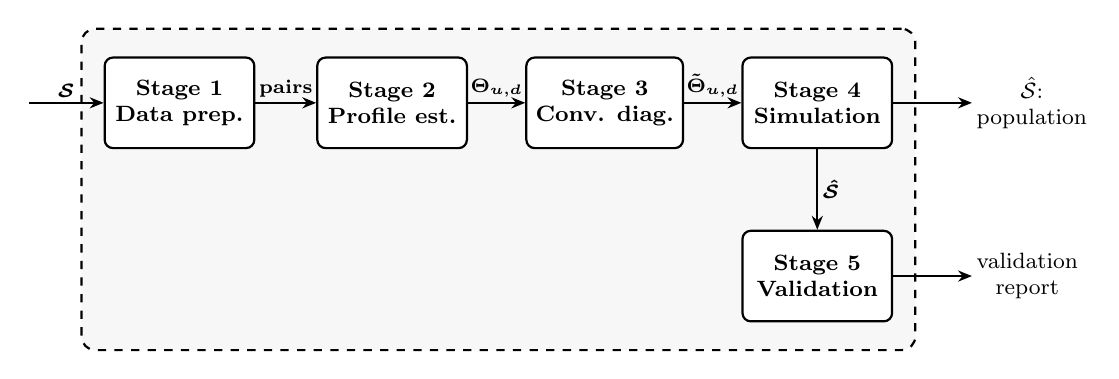
\begin{tikzpicture}[
  stage/.style={rectangle, rounded corners=3pt, draw, thick, fill=white,
                minimum width=1.9cm, minimum height=1.15cm, align=center,
                font=\footnotesize\bfseries},
  arr/.style={-{Stealth[length=5pt, width=4pt]}, thick},
  dlbl/.style={font=\scriptsize\bfseries\boldmath, inner sep=1.5pt},
  io/.style={font=\footnotesize, align=center, inner sep=1.5pt},
]
\node[stage] (s1) at (0,0)    {Stage 1\\Data prep.};
\node[stage] (s2) at (2.7,0)  {Stage 2\\Profile est.};
\node[stage] (s3) at (5.4,0)  {Stage 3\\Conv. diag.};
\node[stage] (s4) at (8.1,0)  {Stage 4\\Simulation};
\node[stage] (s5) at (8.1,-2.2) {Stage 5\\Validation};
\begin{scope}[on background layer]
  \node[draw, thick, dashed, rounded corners=5pt, fill=black!3,
        inner xsep=8pt, inner ysep=10pt, fit=(s1)(s4)(s5)] (box) {};
\end{scope}
\draw[arr] ($(s1.west)-(0.95,0)$) -- (s1.west) node[dlbl, above, midway]{$\mathcal{S}$};
\draw[arr] (s1) -- (s2) node[dlbl, above, midway]{pairs};
\draw[arr] (s2) -- (s3) node[dlbl, above, midway]{$\Theta_{u,d}$};
\draw[arr] (s3) -- (s4) node[dlbl, above, midway]{$\tilde{\Theta}_{u,d}$};
\node[io, right=1.0cm of s4] (pop) {$\hat{\mathcal{S}}$:\\population};
\draw[arr] (s4.east) -- (pop.west);
\draw[arr] (s4.south) -- (s5.north) node[dlbl, right, midway]{$\hat{\mathcal{S}}$};
\node[io, right=1.0cm of s5] (rep) {validation\\report};
\draw[arr] (s5.east) -- (rep.west);
\end{tikzpicture}%
}
\caption{Overview of the SPARC framework. Stages~1--4 transform observed sessions $\mathcal{S}$ into a synthetic population $\hat{\mathcal{S}}$; Stage~5 validates $\hat{\mathcal{S}}$, producing a report.}
\label{fig:framework-overview}
\end{figure}

% Block diagram of Stages 2 and 3 -- equal-size top-aligned stage boxes,
% boundary-to-boundary inter-stage arrow. Requires: \usetikzlibrary{arrows.meta, backgrounds, calc}
\begin{figure}[t]
\centering
\resizebox{0.92\columnwidth}{!}{%
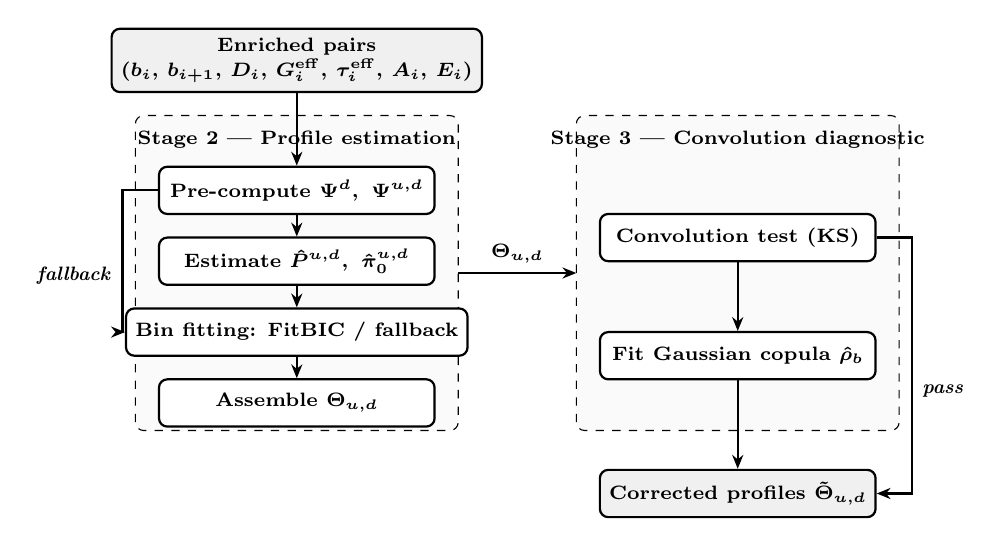
\begin{tikzpicture}[
    box/.style       = {rectangle, rounded corners=3pt, thick, minimum width=3.5cm,
                        minimum height=0.6cm, align=center, font=\scriptsize\bfseries\boldmath,
                        draw=black, fill=white},
    titlenode/.style = {font=\scriptsize\bfseries, text centered},
    iobox/.style     = {box, font=\scriptsize\bfseries\boldmath, fill=black!6},
    lbl/.style       = {font=\scriptsize\bfseries\boldmath},
    arr/.style       = {-{Stealth[length=5pt, width=4pt]}, thick},
]
%% ---- equal-size, top-aligned dashed stage containers ----
\begin{scope}[on background layer]
  \draw[dashed, rounded corners=3pt, fill=black!2] (-2.05,0.25) rectangle (2.05,4.25);
  \draw[dashed, rounded corners=3pt, fill=black!2] ( 3.55,0.25) rectangle (7.65,4.25);
\end{scope}
%% ---- Stage 2 (left): title + 4 blocks, 0.9 spacing (0.3 gaps) ----
\node[titlenode] (s2title)   at (0,3.95) {Stage 2 --- Profile estimation};
\node[box]       (fallback)  at (0,3.30) {Pre-compute $\Psi^d,\ \Psi^{u,d}$};
\node[box]       (jumpchain) at (0,2.40) {Estimate $\hat{P}^{u,d},\ \hat{\pi}_0^{u,d}$};
\node[box]       (binfit)    at (0,1.50) {Bin fitting: \textsc{FitBIC} / fallback};
\node[box]       (assemble)  at (0,0.60) {Assemble $\Theta_{u,d}$};
%% ---- Stage 3 (right): title + 2 blocks, centred with wider gap ----
\node[titlenode] (s3title)  at (5.6,3.95) {Stage 3 --- Convolution diagnostic};
\node[box]       (convtest) at (5.6,2.70) {Convolution test (KS)};
\node[box]       (copula)   at (5.6,1.20) {Fit Gaussian copula $\hat{\rho}_b$};
%% ---- I/O blocks, separated from the stage boxes ----
\node[iobox] (input)  at (0,4.95)   {Enriched pairs\\[1pt] $(b_i,\, b_{i+1},\, D_i,\, G_i^{\mathrm{eff}},\, \tau_i^{\mathrm{eff}},\, A_i,\, E_i)$};
\node[iobox] (output) at (5.6,-0.55) {Corrected profiles $\tilde{\Theta}_{u,d}$};
%% ---- internal chains ----
\draw[arr] (input)     -- (fallback);
\draw[arr] (fallback)  -- (jumpchain);
\draw[arr] (jumpchain) -- (binfit);
\draw[arr] (binfit)    -- (assemble);
\draw[arr] (convtest)  -- (copula);
\draw[arr] (copula)    -- (output);
%% ---- inter-stage arrow: boundary to boundary at box centre ----
\draw[arr] (2.05,2.25) -- (3.55,2.25) node[lbl, midway, above]{$\Theta_{u,d}$};
%% ---- bypasses on the outer sides ----
\draw[arr] (convtest.east) -- ++(0.45,0)
     |- node[lbl, right, pos=0.30]{\textit{pass}} (output.east);
\draw[arr] (fallback.west) -- ++(-0.45,0)
     |- node[lbl, left, pos=0.30]{\textit{fallback}} (binfit.west);
\end{tikzpicture}%
}
\caption{Block diagram of Stages~2 and~3.}
\label{fig:stages23}
\end{figure}


\begin{remark}[Why not a plain Markov chain?]
\label{rem:dtmc-limitation}
A time-indexed DTMC advances on the clock, not on events, so it can start a session before the previous one ends, violating temporal validity~(P3). A CTMC forces exponential sojourns, which is empirically false: a user idle for $30$~h is far likelier to charge next hour than one idle for $4$~h. An arbitrary $F_b$ captures this memory~(P4) while keeping the Markov structure at jump instants.
\end{remark}

\subsection{State Representation}
\label{subsec:state-representation}

The key design choice is what a state represents, since this fixes the temporal structure $P$ can encode. A two-state chain $\mathcal{B} = \{\text{Charging},\, \text{Idle}\}$, with sojourns $D_i$ and $G_i$~\cite{iversen2016inhomogeneous}, is simple but carries little structure: its jump matrix is deterministic and says nothing about \emph{when} sessions occur. We instead take the state to be the time-of-day bin of the current session, $X_i = b(A_i)$, with $b(\cdot)$ from~\eqref{eq:bin-index}. The chain then jumps only at session starts, the state records \emph{when} in the day the user charged, and the sojourn $\sigma_i = \tau_i$ is the time until the next session. Consequently $P(b, b')$, the probability that a session in bin $b$ is followed by one in bin $b'$, directly encodes the user's routine; self-transitions (evening charging on consecutive days) are expected and handled by construction. Because the chain advances on events, not the clock, it cannot conflate elapsed time with a charging decision or emit overlapping sessions (Remark~\ref{rem:dtmc-limitation}).


\section{Problem Formulation}
\label{sec:problem-formulation}

Let $\mathcal{U} = \{1, 2, \ldots, N_u\}$ be a population of EV users, where a \emph{user} is any recurring charging identity (a resident, a commuter, or a commercial account), not necessarily a distinct individual. Each user contributes a chronologically ordered sequence of $n_u$ sessions $\mathcal{S}_u = \bigl\{(u,\, T_i^{\mathrm{start}},\, D_i,\, E_i)\bigr\}_{i=1}^{n_u}$ (Section~\ref{subsec:session-random-object}); the dataset is $\mathcal{S} = \bigcup_{u} \mathcal{S}_u$ with $n = \sum_{u} n_u$ sessions. The problem is to estimate, for each user $u$ and day-type $d \in \mathcal{D}$~(P1,~P3), a compact, interpretable tuple
\begin{IEEEeqnarray}{rCl}
    \Theta_{u,d} & = & \bigl(
    \pi_0^{u,d},\; P^{u,d},\;
    \{\mathcal{D}_b^{u,d}\}_{b=1}^{B},\nonumber\\
    && \{\mathcal{G}_b^{u,d}\}_{b=1}^{B},\;
    \{\mathcal{E}_b^{u,d}\}_{b=1}^{B},\;
    \{\mathcal{A}_b^{u,d}\}_{b=1}^{B}
    \bigr).
    \label{eq:profile-tuple}
\end{IEEEeqnarray}
Here $\pi_0^{u,d} \in \Delta^{B-1}$ is the initial bin distribution, $P^{u,d} \in [0,1]^{B \times B}$ the row-stochastic jump matrix over bins~(P2), and $\mathcal{D}_b^{u,d}, \mathcal{G}_b^{u,d}, \mathcal{E}_b^{u,d}, \mathcal{A}_b^{u,d}$ the per-bin CDFs of plug-in duration, idle gap, energy, and arrival time, drawn from non-exponential families~(P4). The tuple must be estimable from the few tens of sessions per user typical of real data~(P5), with the same form across residential, workplace, and commercial settings~(P6). From $\Theta_{u,d}$, for any horizon $H > 0$ and start date $t_0$, a synthetic sequence $\hat{\mathcal{S}}_u = \bigl\{(u,\, \hat{T}_i^{\mathrm{start}},\, \hat{D}_i,\, \hat{E}_i)\bigr\}_{i=1}^{\hat{n}_u}$ is drawn that is statistically and temporally consistent with $\mathcal{S}_u$~(P3); the horizon, start date, and user set are free parameters, so populations can be resized or recomposed at will~(P7), and $\hat{\mathcal{S}} = \bigcup_{u} \hat{\mathcal{S}}_u$.

The framework succeeds for user $u$ if $\hat{\mathcal{S}}_u$ passes all four levels of the validation protocol of Section~\ref{subsec:stage5}: \emph{L1}, the marginals of $A$, $D$, $G^{\mathrm{eff}}$, and $E$; \emph{L2}, the bin-to-bin transitions; \emph{L3}, the sojourn distribution; and \emph{L4}, the population-level KL divergence ($\mathrm{KL}_v \leq \epsilon$). This per-user criterion is deliberately stronger than the population-level fit by which pooled generators are judged. A population session is drawn in two stages, first a user $u$, then a session from that user's own law; writing $\mu_u = \mathbb{E}[X \mid u]$ for a session variable $X$, the law of total variance splits the population spread accordingly,
\begin{equation}
    \mathrm{Var}(X) =
    \underbrace{\mathbb{E}_u\!\left[\mathrm{Var}(X \mid u)\right]}_{\text{within-user}}
    + \underbrace{\mathrm{Var}_u\!\left(\mu_u\right)}_{\text{between-user}},
    \label{eq:total-variance}
\end{equation}
into each user's session-to-session spread and the spread of personal habits across users. A pooled generator preserves the total while giving all users one common law: the between-user term collapses to zero and its share is reallocated within users, making every synthetic user an average user behind a perfect population histogram. Passing L1--L3 \emph{per user} certifies the between-user term; L4 then confirms the population mixture follows. The reverse implication does not hold.

\section{The Proposed Framework}
\label{sec:framework}

We now present SPARC, the per-user semi-Markov framework that solves this problem (Fig.~\ref{fig:framework-overview}). It factorizes the population by user and day-type, fitting a dedicated SMC per profile $(u,d)$ with the session-as-state encoding of Section~\ref{subsec:state-representation}, so each profile retains its own temporal structure~(P1) and weekday/weekend shift~(P3). The framework is modular: any stage is independently replaceable; for instance, the Stage~2 density estimator can be swapped for any parametric, non-parametric, or learned alternative without affecting the others. The remainder of this section details its five stages: data preparation, profile estimation, convolution diagnostic, simulation, and validation.

\begin{remark}[Scope]
\label{rem:scope}
SPARC requires recurring, identifiable users, applying wherever sessions attach to persistent identities with habitual routines. It is not intended for anonymous, one-off public charging, where sessions cannot be linked into per-user histories~\cite{jonas2023electric}.
\end{remark}

\subsection{Stage 1: Data Preparation}
\label{subsec:stage1}

Stage~1 converts raw session records into a clean set of consecutive same-day-type session pairs. We first apply dataset-level filtering, retaining a session only if its energy exceeds a threshold $E_{\min}$ (removing aborted sessions) and its plug-in duration lies within $[D_{\min},\, D_{\max}]$ (removing spurious connections and pathological outliers); sessions from atypical periods, such as pandemic lockdowns~\cite{palomino2021impact}, are also excluded, since such disruptions break the habitual routines the framework learns. We then filter at the user level, retaining a user $u$ with $n_u$ sessions only when $n_{\min} \le n_u < n_{\max}$. Here $n_{\min}$ is the minimum count for stable per-bin fitting in Stage~2, while the upper cutoff $n_{\max} = Q_q(\{n_u\})$ is the $q$-th percentile of the per-user session-count distribution, not a fixed constant, so it adapts to each dataset and trims only a small upper tail of atypically active users. Both are dataset-specific (Section~\ref{sec:case-study}).

For each retained user $u$ and day-type $d$, consecutive same-type sessions are sorted and paired, each pair yielding the inter-arrival $\tau_i$ and its split into plug-in duration $D_i$ and idle gap $G_i$ (Section~\ref{subsec:session-random-object}). Because the weekday and weekend processes are modeled independently, sojourns are measured in \emph{effective same-type time}, i.e.\ calendar time restricted to hours of day-type $d$. The effective idle gap is $G_i^{\mathrm{eff}} \triangleq \int_{T_i^{\mathrm{end}}}^{T_{i+1}^{\mathrm{start}}} \mathbf{1}_{\{\mathrm{dt}(s) = d\}}\, \mathrm{d}s$ (hours), and the effective inter-arrival is $\tau_i^{\mathrm{eff}} \triangleq D_i + G_i^{\mathrm{eff}}$. For instance, a weekday gap spanning Friday~18:00 to Monday~09:00 contributes $G_i^{\mathrm{eff}} = 15$~hours rather than the raw $63$~hours, since the $48$ intervening weekend hours are invisible to the weekday process. Stage~1 outputs, for each profile $(u, d)$, the enriched pairs $\bigl(b_i,\, b_{i+1},\, D_i,\, G_i^{\mathrm{eff}},\, \tau_i^{\mathrm{eff}},\, A_i,\, E_i\bigr)$, which feed Stage~2.

\subsection{Stage 2: Profile Estimation}
\label{subsec:stage2}

From the enriched pairs, Stage~2 estimates the profile tuple $\Theta_{u,d}$ in two steps. First, the jump matrix $P^{u,d}$ and initial distribution $\pi_0^{u,d}$ are obtained directly from the observed transition counts. Second, for each bin and quantity $x \in \{D, G^{\mathrm{eff}}, E, A\}$, a candidate distribution is fit by maximum likelihood and selected by the Bayesian Information Criterion (BIC)~\cite{zhang2023information}, with a hierarchical fallback for bins too sparse to fit directly.

\subsubsection{Embedded jump matrix and initial distribution}

We estimate $P^{u,d}$ from the observed bin-to-bin transition counts, Laplace-smoothed by a pseudo-count $\alpha$ (equivalently, the posterior mean under a symmetric $\mathrm{Dirichlet}(\alpha)$ prior)~\cite{bazille2020global}:
\begin{equation}
    \hat{P}^{u,d}(b,\, b') =
    \frac{N_{bb'}^{u,d} + \alpha}
         {\displaystyle\sum_{b''=1}^{B} N_{bb''}^{u,d} + B\alpha},
    \label{eq:jump-matrix-est}
\end{equation}
where $N_{bb'}^{u,d} = \sum_i \mathbf{1}_{\{b_i = b,\, b_{i+1} = b'\}}$ counts transitions from bin $b$ to bin $b'$ and $\alpha > 0$. Without smoothing, an unobserved transition $b \to b'$ would receive zero probability, permanently blocking that transition in simulation even if it is physically plausible. In practice each user occupies only a few bins, so $\hat{P}^{u,d}$ is highly sparse and effectively low-dimensional, and this smoothing keeps its estimation stable under the few tens of sessions typical per user~(P5).

The initial bin distribution $\hat{\pi}_0^{u,d}(b)$ is estimated identically, replacing the transition counts $N_{bb'}^{u,d}$ in~\eqref{eq:jump-matrix-est} with the per-bin session counts $M_b^{u,d} = \sum_i \mathbf{1}_{\{b_i = b\}}$.


\subsubsection{Distribution fitting and hierarchical fallback}

For each bin $b$ and quantity $x \in \{D, G^{\mathrm{eff}}, E, A\}$, the marginal is chosen by BIC from a fixed candidate set: three unimodal families and a truncated Gaussian mixture~\cite{zhao2019variational},
\begin{align}
    \text{LogNormal}(\mu, \sigma)\!: \quad
    &f(x) = \frac{1}{x\sigma\sqrt{2\pi}}
    \exp\!\left(-\frac{(\ln x - \mu)^2}{2\sigma^2}\right),
    \nonumber \\
    \text{Exponential}(\theta)\!: \quad
    &f(x) = \frac{1}{\theta}\, e^{-x/\theta},
    \nonumber \\
    \text{Weibull}(k, \lambda)\!: \quad
    &f(x) = \frac{k}{\lambda}
    \left(\frac{x}{\lambda}\right)^{k-1}
    e^{-(x/\lambda)^k},
    \nonumber \\
    \text{Truncated GMM}\!: \quad
    &f(x) = \sum_{k=1}^{K} w_k\,
    \mathcal{TN}(x;\, \mu_k,\, \sigma_k^2,\, 0,\, x_{\max}),
    \label{eq:candidate-families}
\end{align}
where $\mathcal{TN}(\cdot;\, \mu, \sigma^2, a, b)$ is $\mathcal{N}(\mu, \sigma^2)$ truncated to $(a, b]$, the weights satisfy $w_k > 0$ and $\sum_{k=1}^{K} w_k = 1$, and $x_{\max} = 2\max_i x_i$ is a heuristic upper bound restricting the mixture to $(0, x_{\max}]$. The number of components $K \in \{1, 2, \ldots, K_{\max}\}$ is capped so that each has at least two observations; the mixture is fit by EM~\cite{lee2012algorithms} with truncation handled in the updates, giving $3K - 1$ free parameters. Each candidate is fit by maximum likelihood, and the one minimizing $\mathrm{BIC} = p \ln n - 2\,\ell$ is selected, where $p$ is its number of free parameters, $\ell = \sum_i \ln f(x_i)$ the maximized log-likelihood, and $n$ the sample size.


\begin{table}[t]
\centering
\caption{Selected cohorts (wd = weekday-only; Profiles = (entity, day-type) models).}
\label{tab:datasets}
\setlength{\tabcolsep}{3pt}
\footnotesize
\begin{tabular}{lllllrrr}
\toprule
\textbf{Dataset} & \textbf{Setting} & \textbf{Reg.} & \textbf{Entity} & \textbf{Days} & \textbf{$N$} & \textbf{Sess.} & \textbf{Profiles} \\
\midrule
Norway~\cite{sorensen2024}   & Resid. & NO & driver  & wd+we & 100 & 22{,}900 & 200 \\
GIST-Res~\cite{baek2024dataset}  & Resid. & KR & driver  & wd+we &  30 &  3{,}059 &  60 \\
GIST-Comm~\cite{baek2024dataset} & Comm.  & KR & driver  & wd    &  25 &  1{,}706 &  25 \\
ACN~\cite{lee2019acndata}        & Workpl.& US & station & wd+we &  15 &  3{,}871 &  30 \\
\midrule
Combined                     & Mixed  & All & mixed & wd+we & 170 & 31{,}536 & 315 \\
\bottomrule
\end{tabular}
\end{table}


\begin{remark}[Choice of candidate families]
\label{rem:family-choice}
The unimodal families cover the shapes common in EV charging data~\cite{flammini2019}: Exponential (memoryless, light-tailed), Weibull (monotone hazard), and LogNormal (right-skewed, over-dispersed, as for plug-in durations). The truncated GMM adds multimodality, for instance a user mixing short opportunistic and long overnight charges in one bin, and BIC selects it only when its extra $3K - 1$ parameters are warranted.
\end{remark}

When a bin has too few observations to fit reliably, its fit falls back through a pre-computed cascade of increasing scope, each bin taking the finest reliable level:
\begin{enumerate}
    \item \emph{Local} (bin-level): the bin's own sample, used if it holds at least $n_{\mathrm{bin}}$ observations;
    \item \emph{Pooled} (user-level): otherwise the user's day-type profile, i.e.\ all bins of that $(u,d)$, used if it holds at least $n_{\mathrm{pool}}$ observations; and
    \item \emph{Global} (dataset-level): otherwise all day-type-$d$ sessions across the dataset.
\end{enumerate}
Since the pooled and global fits are computed once and shared, none is refit. The output of Stage~2 is the fitted profile set $\boldsymbol{\Theta} = \{\Theta_{u,d}\}_{u,d}$, passed to Stage~3.

\begin{remark}[Fallback bins are rarely visited]
\label{rem:fallback-weight}
Bins requiring fallback are, by construction, sparsely populated: few sessions start in them and few transitions lead into them, so both the initial distribution $\hat{\pi}_0^{u,d}$ and the transition matrix $\hat{P}^{u,d}$ place little mass on them. They are therefore seldom visited during simulation, and their coarser fits have negligible effect on the output.
\end{remark}

\subsection{Stage 3: Convolution Diagnostic and Distribution Update}
\label{subsec:stage3}

The simplification $F_{bb'} = F_b$ (Section~\ref{subsec:smc-formal-def}) makes the sojourn $\tau_i^{\mathrm{eff}} = D_i + G_i^{\mathrm{eff}}$ independent of the destination bin $b'$; a sufficient condition is $D_i \perp G_i^{\mathrm{eff}}$ given $b$, so the sojourn density factorizes as the convolution of the two marginals. Stage~3 tests this per bin and, where it fails, fits a Gaussian copula for the residual $D$--$G$ dependence.






\subsubsection{Convolution test}

For each bin $b$ with at least $n_{\mathrm{bin}}$ pairs, we test whether the observed $\tau_i^{\mathrm{eff}}$ matches the convolution of the fitted marginals $\mathcal{D}_b$ and $\mathcal{G}_b$. We draw $N_{\mathrm{sim}}$ independent paired samples $d_k^{\mathrm{sim}} \sim \mathcal{D}_b$, $g_k^{\mathrm{sim}} \sim \mathcal{G}_b$, $\tau_k^{\mathrm{sim}} = d_k^{\mathrm{sim}} + g_k^{\mathrm{sim}}$, and compare $\{\tau_k^{\mathrm{sim}}\}$ with the empirical $\{\tau_j^{\mathrm{eff}}\}$ via the two-sample Kolmogorov--Smirnov statistic
\begin{equation}
    \mathrm{KS} = \sup_x \left| \hat{F}^{\mathrm{sim}}(x) - \hat{F}^{\mathrm{emp}}(x) \right|.
    \label{eq:ks-statistic}
\end{equation}
The bin passes if the KS $p$-value exceeds $\alpha_{\mathrm{KS}} = 0.05$; a failing bin signals $D$--$G^{\mathrm{eff}}$ dependence and receives the copula correction below. For reporting, we additionally flag a failing bin as \emph{correlated} when the Pearson or Spearman correlation of $\{d_i\}$ and $\{g_i\}$ exceeds $0.3$ in magnitude. The two criteria are complementary: the convolution KS test detects any $D$--$G^{\mathrm{eff}}$ dependence, including nonlinear, whereas the correlations quantify only its linear part.

\begin{remark}[Physical interpretation of $D$--$G$ correlation]
\label{rem:dg-correlation}
Within-bin $D$--$G^{\mathrm{eff}}$ correlation arises mainly from battery state of charge (SoC): a short session leaves the battery depleted, shortening the gap to the next charge, whereas a long session refills it, lengthening the gap. This positive correlation is usually weak relative to the time-of-day effect, so the independence factorization remains an acceptable first-order approximation for most bins.
\end{remark}


\begin{table*}[t]
\centering
\caption{Four-level validation: L1--L3 per-profile pass rates (\%), L4 population KL (nats); mean$\pm$std over five seeds.}
\label{tab:validation}
\setlength{\tabcolsep}{4pt}
\footnotesize
\begin{tabular}{ll cccc cc cccc}
\toprule
\multirow{2}{*}{\textbf{Dataset}} & \multirow{2}{*}{\textbf{Entity}} & \multicolumn{4}{c}{\textbf{L1 (per-user), \%}} & \textbf{L2} & \textbf{L3} & \multicolumn{4}{c}{\textbf{L4 (KL, nats)}} \\
\cmidrule(lr){3-6}\cmidrule(lr){9-12}
 & & $A$ & $D$ & $G$ & $E$ & {\footnotesize(transition)} & {\footnotesize(sojourn)} & $A$ & $D$ & $G$ & $E$ \\
\midrule
Norway & driver & $81.7\pm2.4$ & $90.5\pm0.7$ & $92.1\pm1.2$ & $97.5\pm0.9$ & $96.1\pm1.0$ & $85.5\pm2.2$ & 0.011 & 0.017 & 0.004 & 0.003 \\
GIST-Res & driver & $83.7\pm2.8$ & $87.8\pm1.6$ & $91.0\pm2.5$ & $93.1\pm1.1$ & $94.5\pm1.6$ & $95.2\pm2.7$ & 0.010 & 0.016 & 0.025 & 0.017 \\
GIST-Comm & driver & $88.8\pm3.0$ & $89.6\pm2.0$ & $99.2\pm1.6$ & $99.2\pm1.6$ & $97.6\pm2.0$ & $93.6\pm2.0$ & 0.023 & 0.033 & 0.069 & 0.031 \\
ACN & station & $84.0\pm2.5$ & $97.3\pm2.5$ & $94.0\pm3.3$ & $95.3\pm3.4$ & $93.3\pm3.0$ & $95.3\pm3.4$ & 0.023 & 0.010 & 0.011 & 0.070 \\
\midrule
Combined & mixed & $82.4\pm1.6$ & $88.8\pm2.0$ & $90.4\pm1.4$ & $96.2\pm0.7$ & $94.4\pm0.7$ & $85.8\pm1.2$ & 0.005 & 0.012 & 0.004 & 0.003 \\
\bottomrule
\end{tabular}
\end{table*}

\subsubsection{Distribution update for failing bins}

For bins that fail the convolution test, we couple $D$ and $G^{\mathrm{eff}}$ with a copula while preserving the Stage-2 marginals. In principle any copula family applies; we use a Gaussian copula~\cite{nelsen2006introduction} for its single interpretable parameter and closed-form sampling. The procedure is as follows:
\begin{enumerate}
    \item Using the marginal CDFs $\mathcal{D}_b$ and $\mathcal{G}_b$ from Stage~2, apply the Probability Integral Transform (PIT) to map per-bin observations to approximate standard normals:
    \begin{equation}
        z_{d,i} = \Phi^{-1}\!\left(\mathcal{D}_b(d_i)\right),
        \qquad
        z_{g,i} = \Phi^{-1}\!\left(\mathcal{G}_b(g_i)\right),
        \label{eq:pit-transform}
    \end{equation}
    where $\Phi^{-1}$ is the standard normal quantile function.
    \item Estimate the latent correlation $\hat{\rho}_b = \widehat{\mathrm{corr}}(z_d, z_g)$.
    \item To draw a joint sample $(d, g)$ during simulation, sample from the bivariate normal
    \begin{equation}
        (z_d, z_g) \sim \mathcal{N}\!\left(\mathbf{0},\,
        \begin{pmatrix} 1 & \hat{\rho}_b \\
        \hat{\rho}_b & 1 \end{pmatrix}\right),
        \label{eq:bivariate-normal}
    \end{equation}
    then back-transform via $d = \mathcal{D}_b^{-1}(\Phi(z_d))$
    and $g = \mathcal{G}_b^{-1}(\Phi(z_g))$.
\end{enumerate}
This approach adds one interpretable scalar $\hat{\rho}_b$ per failing bin while leaving all marginal distributions intact. The output of Stage~3 is the corrected profile $\tilde{\Theta}_{u,d}$, identical to $\Theta_{u,d}$ except that failing bins carry the fitted $\hat{\rho}_b$ for use in Stage~4. The block diagram of Stage~2 and Stage~3 is shown in Fig.~\ref{fig:stages23}.

\begin{remark}[Which dependences are corrected, and which are not]
\label{rem:which-dependence}
Only the $D$--$G^{\mathrm{eff}}$ pair is coupled, because only these two enter the sojourn $\tau^{\mathrm{eff}} = D + G^{\mathrm{eff}}$ that moves the chain forward in time. Energy $E$ and arrival $A$ do not affect the timing and are drawn from their own per-bin distributions; conditioning on the time-of-day bin already absorbs their main common driver, the hour of the day. The correction is thus targeted and interpretable: dependence is added only where the convolution test detects it, at the cost of a single parameter per failing bin, and any dependence left unmodeled involves energy only, so it cannot alter when sessions occur. A richer joint over $(A, D, G^{\mathrm{eff}}, E)$, e.g.\ a vine copula within the same modular Stage~3, is future work.
\end{remark}


\subsection{Stage 4: Simulation}
\label{subsec:stage4}

Stage~4 draws synthetic sessions from the corrected profiles $\tilde{\boldsymbol{\Theta}}$. For each user $u$ and day-type $d$, a renewal process runs on an effective-time clock over a horizon $H$ from an anchor date $t_0$. The horizon, anchor, and session count are configurable per user, supporting historical replay, a common horizon, or counterfactual future scenarios~(P7). Per user and day-type, the stream starts at $b \sim \hat{\pi}_0^{u,d}$ and repeats until the same-type budget is exhausted: draw $D \sim \mathcal{D}_b$ and $G \sim \mathcal{G}_b(\cdot \mid D)$, advance the effective clock by $D + G$, map to calendar time via $\Phi_d$, draw $E \sim \mathcal{E}_b$ and $A \sim \mathcal{A}_b$, emit the session, and jump to $b' \sim P^{u,d}(b, \cdot)$; the weekday and weekend streams run on separate clocks and are merged into $\hat{\mathcal{S}}_u$.


Here the conditional draw $\mathcal{G}_b(\cdot \mid D)$ reduces to the marginal $\mathcal{G}_b$ for bins that passed Stage~3 and uses the fitted copula otherwise, and the effective-to-calendar map $\Phi_d(t^{\mathrm{eff}}, t_0)$ returns the smallest calendar time $t \geq t_0$ at which exactly $t^{\mathrm{eff}}$ hours of day-type $d$ have elapsed since $t_0$. The division of labor is deliberate: the effective clock and $\Phi_d$ fix the calendar \emph{day} of each session, while its time of day is drawn from the bin's arrival law $\mathcal{A}_b$, keeping the arrival consistent with the state $b$.

\emph{Worked example.} Let $w = 2$~h ($B = 12$), anchor $t_0 = $ Monday 00:00, weekday stream, effective clock at $t^{\mathrm{eff}} = 97.0$~h, current state $b = 9$ (the $[16{:}00, 18{:}00)$ bin). One simulation step: (i)~draw $D = 12.4$~h from $\mathcal{D}_9$; bin~9 failed Stage~3 with $\hat{\rho}_9 = 0.42$, so $G = 21.1$~h is drawn from the copula conditional $\mathcal{G}_9(\cdot \mid D)$; (ii)~advance the clock by $\tau^{\mathrm{eff}} = D + G = 33.5$~h to $t^{\mathrm{eff}} = 130.5$~h; (iii)~map to calendar: the first $120$ weekday-hours exhaust Monday--Friday, so the residual $10.5$~h lands on the \emph{following} Monday at 10:30, the weekend being invisible to the weekday clock; (iv)~draw $E = 8.6$~kWh from $\mathcal{E}_9$ and $A = 17.3$ from $\mathcal{A}_9$, so the session starts that Monday at 17:18 and runs $12.4$~h; (v)~jump to $b' \sim P^{u,\mathrm{wd}}(9, \cdot)$, here the self-transition of an evening routine. The weekend stream evolves on its own clock and budget, and the two streams are merged by calendar date.

\subsection{Stage 5: Validation}
\label{subsec:stage5}

Stage~5 evaluates $\hat{\mathcal{S}}$ against the real sessions using the four-level hierarchical protocol of Section~\ref{sec:problem-formulation}, built on standard two-sample tests~\cite{lehmann2005testing}. A profile is included in reporting only if it has at least $n_{\mathrm{obs}}$ sessions in both the real and simulated sets.

\emph{L1: Marginal distributions.} For each profile $(u,d)$ and each variable $v \in \{A, D, G^{\mathrm{eff}}, E\}$, a two-sample KS test~\eqref{eq:ks-statistic} compares the real and simulated marginals, passing if the $p$-value exceeds $\alpha_{\mathrm{KS}} = 0.05$.

\emph{L2: Transition matrix.} The bin-to-bin transition structure of each profile $(u,d)$ is tested via a Pearson $\chi^2$ test. Both the real and simulated count matrices are Laplace-smoothed with $\alpha = 10^{-4}$ before testing. For each source bin $b$, the expected count under the real row-normalized transition probabilities is $E_{bb'} = \hat{P}^{\mathrm{real}}(b, b') \cdot \sum_{b''} N_{bb''}^{\mathrm{sim}}$, and the test statistic is
\begin{equation}
    \chi^2 = \sum_{\substack{b,\, b':\\ E_{bb'} \geq 0.5}}
    \frac{\left(N_{bb'}^{\mathrm{sim}} - E_{bb'}\right)^2}
         {E_{bb'}}.
    \label{eq:l2-chi2}
\end{equation}
Cells with $E_{bb'} < 0.5$ are excluded, since near-zero expected counts break the $\chi^2$ approximation and would inflate the statistic.

\emph{L3: Sojourn time distribution.} For each profile $(u, d)$, a two-sample KS test~\eqref{eq:ks-statistic} compares the real $\tau_i^{\mathrm{eff}}$ distribution against the simulated inter-arrival times, passing if the $p$-value exceeds $\alpha_{\mathrm{KS}}$. This directly tests the fitted sojourn model (the core of the SMC) and, unlike count-based comparisons, is unaffected by any mismatch between the simulated horizon $H$ and the real observation window.

\emph{L4: Population-level distributions.} All sessions from $\hat{\mathcal{S}}$ and $\mathcal{S}$ are compared at the population level for each variable $v \in \{A, D, G^{\mathrm{eff}}, E\}$. Arrival hours are binned into 24 clock-hour bins; the remaining variables are binned into 50 equal-width bins with Laplace smoothing. Each pair of histograms is normalized to probability mass functions $P_v^{\mathrm{real}}$ and $P_v^{\mathrm{sim}}$, and the KL divergence is computed as
\begin{equation}
    \mathrm{KL}_v(P_v^{\mathrm{real}} \| P_v^{\mathrm{sim}}) =
    \sum_{k} P_v^{\mathrm{real}}(k)
    \ln \frac{P_v^{\mathrm{real}}(k) + \delta}
             {P_v^{\mathrm{sim}}(k) + \delta},
    \label{eq:kl-l4}
\end{equation}
where $\delta = 10^{-9}$. As a guideline, $\mathrm{KL}_v$ below $0.05$~nats indicates excellent agreement, $0.05$--$0.15$~nats is acceptable, and above $0.15$~nats a significant discrepancy; we therefore set the L4 tolerance $\epsilon = 0.15$~nats. The protocol constants guard test validity rather than tune results: $\alpha_{\mathrm{KS}} = 0.05$ is conventional, the $\chi^2$ cell floor protects the asymptotic approximation, and $\epsilon$ is the acceptable-band boundary. Each user is simulated over its own observation window, so real and simulated per-profile sample sizes are comparable at L1--L2, and L3 is horizon-invariant by construction. Distance-based evaluation of synthetic smart-grid data is an active research direction in its own right~\cite{cai2026frechet}; Section~\ref{subsec:validation-results} reports binning-free distances alongside the tests.

%%%%%%%%%%%%%%%%%%%%%%%%%%%%%%%%%%%%%%
%%%%%%%%%%%%%%%%%%%%%%%%%%%%%%%%%%%%%%

%%%%%%%%%%%%%%%%%%%%%%%%%%%%%%%%%%%%%%
%%%%%%%%%%%%%%%%%%%%%%%%%%%%%%%%%%%%%%

\section{Case Study}
\label{sec:case-study}





\begin{figure*}[t]
  \centering
  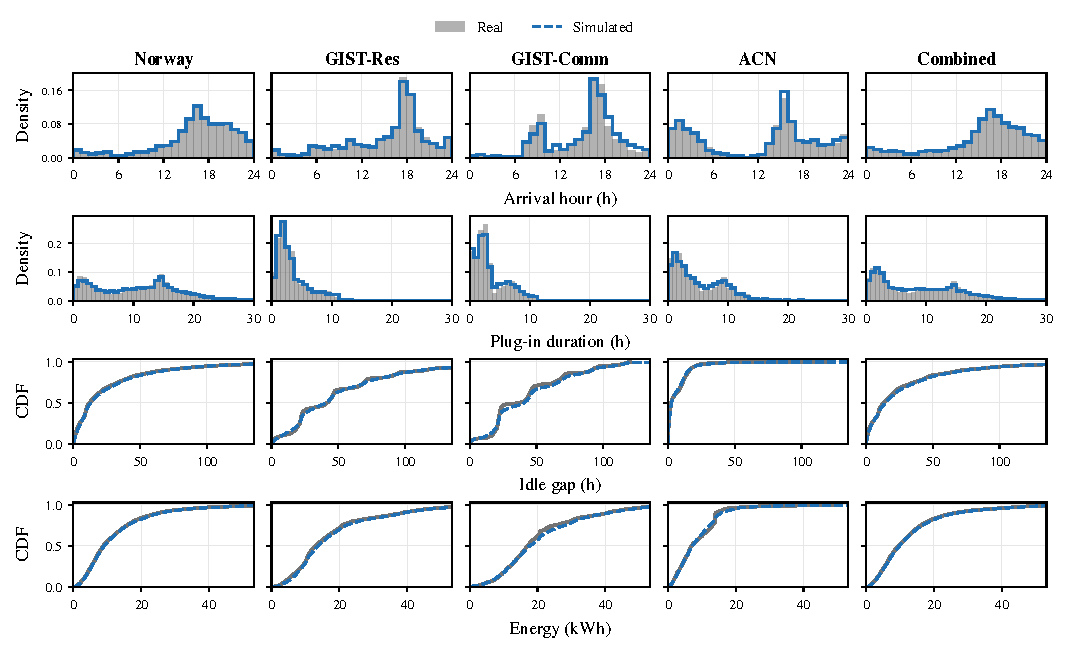
\includegraphics[width=0.91\textwidth]{figures/fig_marginals_grid.pdf}
  \caption{Population marginals, real (gray) vs.\ simulated (blue): arrival and duration (density); idle gap and energy (CDF).}
  \label{fig:marginals}
\end{figure*}

\begin{table}[t]
\centering
\caption{Aggregate marginal fidelity: forward KL (nats), mean$\pm$std; best per column in bold.}
\label{tab:benchmark}
\setlength{\tabcolsep}{4pt}
\footnotesize
\begin{tabular}{llccc}
\toprule
Dataset & Method & $A$ & $D$ & $E$ \\
\midrule
Norway & SPARC & 0.011$\pm$0.000 & 0.021$\pm$0.002 & 0.002$\pm$0.000 \\
 & Copula & \textbf{0.001$\pm$0.000} & \textbf{0.001$\pm$0.000} & \textbf{0.001$\pm$0.000} \\
 & GMMNet & 0.019$\pm$0.001 & 0.080$\pm$0.003 & 0.043$\pm$0.002 \\
 & EV-SDG & 0.162$\pm$0.007 & 17.9$\pm$0.0 & 2.357$\pm$0.005 \\
\midrule
GIST-Res & SPARC & \textbf{0.010$\pm$0.002} & 0.023$\pm$0.002 & 0.013$\pm$0.002 \\
 & Copula & 0.012$\pm$0.009 & \textbf{0.012$\pm$0.007} & \textbf{0.011$\pm$0.003} \\
 & GMMNet & 0.065$\pm$0.008 & 0.049$\pm$0.006 & 0.055$\pm$0.010 \\
 & EV-SDG & 0.397$\pm$0.024 & 0.129$\pm$0.009 & 4.199$\pm$0.036 \\
\midrule
GIST-Comm & SPARC & \textbf{0.023$\pm$0.001} & 0.031$\pm$0.005 & 0.023$\pm$0.003 \\
 & Copula & 0.035$\pm$0.023 & \textbf{0.015$\pm$0.003} & \textbf{0.013$\pm$0.003} \\
 & GMMNet & 0.155$\pm$0.013 & 0.198$\pm$0.047 & 0.123$\pm$0.011 \\
 & EV-SDG & 0.838$\pm$0.019 & 0.260$\pm$0.010 & 6.078$\pm$0.004 \\
\midrule
ACN & SPARC & 0.023$\pm$0.004 & \textbf{0.021$\pm$0.008} & 0.078$\pm$0.010 \\
 & Copula & \textbf{0.006$\pm$0.005} & 0.027$\pm$0.016 & 0.075$\pm$0.015 \\
 & GMMNet & 0.085$\pm$0.007 & 0.033$\pm$0.014 & \textbf{0.057$\pm$0.011} \\
 & EV-SDG & 0.391$\pm$0.007 & 0.160$\pm$0.004 & 0.432$\pm$0.005 \\
\midrule
Combined & SPARC & 0.005$\pm$0.001 & 0.014$\pm$0.001 & 0.003$\pm$0.000 \\
 & Copula & \textbf{0.001$\pm$0.000} & \textbf{0.001$\pm$0.000} & \textbf{0.001$\pm$0.000} \\
 & GMMNet & 0.012$\pm$0.001 & 0.024$\pm$0.001 & 0.018$\pm$0.001 \\
 & EV-SDG & 0.173$\pm$0.011 & 13.3$\pm$0.6 & 2.335$\pm$0.006 \\
\bottomrule
\end{tabular}
\end{table}
\begin{table}[t]
\centering
\caption{Structure the marginals miss: across-user SD (h) of mean arrival hour and duration (closest to \emph{Real} in bold); KL of the 24\,h load shape.}
\label{tab:heterogeneity}
\footnotesize
\begin{tabular}{llccc}
\toprule
Dataset & Method & $\sigma_A$ & $\sigma_D$ & $D_{\mathrm{KL}}^{L}$ \\
\midrule
Norway & Real & 2.03$\pm$0.00 & 5.66$\pm$0.00 & -- \\
 & SPARC & \textbf{2.16$\pm$0.03} & \textbf{5.46$\pm$0.13} & \textbf{0.025$\pm$0.001} \\
 & Copula & 0.32$\pm$0.02 & 0.89$\pm$0.08 & 0.049$\pm$0.001 \\
 & GMMNet & 0.36$\pm$0.03 & 0.97$\pm$0.08 & 0.030$\pm$0.001 \\
 & EV-SDG & 0.85$\pm$0.16 & 0.08$\pm$0.02 & 0.088$\pm$0.007 \\
\midrule
GIST-Res & Real & 3.61$\pm$0.00 & 1.90$\pm$0.00 & -- \\
 & SPARC & \textbf{3.43$\pm$0.03} & \textbf{1.85$\pm$0.05} & \textbf{0.007$\pm$0.001} \\
 & Copula & 0.44$\pm$0.07 & 0.25$\pm$0.03 & 0.054$\pm$0.008 \\
 & GMMNet & 0.48$\pm$0.06 & 0.25$\pm$0.03 & 0.080$\pm$0.010 \\
 & EV-SDG & 3.33$\pm$0.47 & 0.28$\pm$0.04 & 0.155$\pm$0.012 \\
\midrule
GIST-Comm & Real & 3.99$\pm$0.00 & 2.16$\pm$0.00 & -- \\
 & SPARC & \textbf{4.15$\pm$0.04} & \textbf{2.15$\pm$0.03} & \textbf{0.009$\pm$0.001} \\
 & Copula & 0.66$\pm$0.12 & 0.33$\pm$0.04 & 0.083$\pm$0.011 \\
 & GMMNet & 1.13$\pm$0.21 & 0.31$\pm$0.04 & 0.034$\pm$0.006 \\
 & EV-SDG & 0.63$\pm$0.12 & 0.26$\pm$0.05 & 0.364$\pm$0.008 \\
\midrule
ACN & Real & 1.73$\pm$0.00 & 1.62$\pm$0.00 & -- \\
 & SPARC & 2.28$\pm$0.05 & \textbf{1.71$\pm$0.12} & \textbf{0.017$\pm$0.002} \\
 & Copula & 0.65$\pm$0.17 & 0.37$\pm$0.06 & 0.042$\pm$0.004 \\
 & GMMNet & 0.47$\pm$0.07 & 0.38$\pm$0.08 & 0.053$\pm$0.004 \\
 & EV-SDG & \textbf{1.39$\pm$0.27} & 0.33$\pm$0.07 & 0.178$\pm$0.004 \\
\midrule
Combined & Real & 2.83$\pm$0.00 & 6.68$\pm$0.00 & -- \\
 & SPARC & \textbf{2.86$\pm$0.04} & \textbf{6.53$\pm$0.07} & \textbf{0.019$\pm$0.001} \\
 & Copula & 0.43$\pm$0.03 & 1.07$\pm$0.06 & 0.032$\pm$0.001 \\
 & GMMNet & 0.48$\pm$0.04 & 1.02$\pm$0.07 & 0.038$\pm$0.002 \\
 & EV-SDG & 1.42$\pm$0.44 & 0.06$\pm$0.02 & 0.046$\pm$0.005 \\
\bottomrule
\end{tabular}
\end{table}

\subsection{Datasets and Setup}
\label{subsec:dataset}


We evaluate SPARC on four cohorts from three open datasets, spanning residential, workplace, and commercial settings. Two come from one large Korean network~\cite{baek2024dataset}, at its residential (GIST-Res) and commercial (GIST-Comm) sites, a same-metering comparison across settings; an unrelated Norwegian residential dataset~\cite{sorensen2024} rules out operator effects. The ACN workplace dataset~\cite{lee2019acndata} is keyed on the \emph{charging station}: SPARC models any repeat-charging entity uniformly.

All cohorts share the Stage~1 preparation of Section~\ref{subsec:stage1}: quality filters ($E_i > 0.5$~kWh, $D_i \in [2~\text{min},\, 120~\text{h}]$) drop aborted and spurious sessions, and consecutive same-day-type sessions are paired, discarding pairs whose effective idle gap exceeds $10$~days. GIST-Comm, being weekday-dominated, is modeled on weekdays only, with weekend profiles built where weekend sessions exist.

Per-entity data is scarce and uneven, so each cohort retains a dataset-specific number of recurring entities with sufficient history for stable fitting (Table~\ref{tab:datasets}); irregular entities are also dropped (top-$2\%$ session-count outliers for Norway, non-location-loyal drivers for GIST-Comm). The \emph{combined} pool merges all four cohorts into $170$ entities ($155$ drivers, $15$ stations), a cross-context, cross-entity stress test.

The coefficient of variation $\sigma_{\tau}/\mu_{\tau}$ of the per-profile sojourn equals $1$ under the exponential a CTMC assumes; across the $315$ combined-pool profiles, $80\%$ depart from unity (median $0.81$), predominantly sub-exponential, justifying the arbitrary $F_b$~(P4).

SPARC is implemented in Julia (\texttt{TruncatedGaussianMixtures.jl} for the mixtures, \texttt{HypothesisTests.jl} for the tests). The arrival-hour resolution is per dataset ($B = 12$ two-hour bins for Norway and ACN, $B = 24$ one-hour bins for the denser Korean cohorts and the combined pool), with $\alpha = 10^{-4}$ and $n_{\mathrm{bin}} = 15$; each user is simulated over its own observation window (up to four years), and all metrics average five seeds.

\subsection{Four-Level Validation}
\label{subsec:validation-results}

Table~\ref{tab:validation} reports the four-level protocol (mean\,$\pm$\,std over five seeds): every L1--L3 pass rate exceeds $81\%$ and every L4 stays at or below $0.07$~nats. Fig.~\ref{fig:marginals} overlays the population marginals: the arrival-hour rhythms (residential evening, workplace morning, commercial midday) and multimodal durations are reproduced, and the idle-gap and energy CDFs are visually indistinguishable. The hierarchical fallback fits every profile even under sparse data (P5), and mean sessions per active day agree across all cohorts (Fig.~\ref{fig:downstream}a).


Strengths are context-dependent: GIST-Comm attains the highest marginals (L1-$G$, L1-$E$ at $99\%$) from its tight routines, Norway the sharpest population fit ($\mathrm{KL}_{\max}=0.017$) from its large sample, and the smaller cohorts sit at $0.02$--$0.07$~nats. Since test power grows with sample size, denser cohorts face a stricter bar, so the rates are a lower bound on agreement. Generality shows twice: the $170$-entity combined pool is fit without per-context tuning yet attains the lowest divergence of all ($\mathrm{KL}_{\max}=0.012$), and the per-station ACN cohort validates as strongly as the per-driver cohorts (L1-$D$ $97\%$, L3 $95\%$), confirming the machinery is entity-agnostic (P6).

\begin{table}[t]
\centering
\caption{Complementary distances, real vs.\ SPARC: JS (nats) and binning-free 1-Wasserstein (physical units); seed variation below the last digit.}
\label{tab:distances}
\setlength{\tabcolsep}{3.5pt}
\footnotesize
\begin{tabular}{lcccccc}
\toprule
 & $\mathrm{JS}_A$ & $\mathrm{JS}_D$ & $\mathrm{JS}_E$ & $W_A$ (h) & $W_D$ (h) & $W_E$ (kWh) \\
\midrule
Norway    & 0.003 & 0.005 & 0.001 & 0.40 & 0.52 & 0.28 \\
GIST-Res  & 0.002 & 0.006 & 0.004 & 0.28 & 0.08 & 0.62 \\
GIST-Comm & 0.006 & 0.007 & 0.009 & 0.40 & 0.14 & 0.83 \\
ACN       & 0.006 & 0.004 & 0.012 & 0.50 & 0.28 & 0.42 \\
Combined  & 0.001 & 0.003 & 0.001 & 0.29 & 0.42 & 0.41 \\
\bottomrule
\end{tabular}
\end{table}

Hypothesis tests return pass/fail at a given power, and KL depends on the binning; Table~\ref{tab:distances} therefore adds two complements: the symmetric, bounded Jensen--Shannon divergence and the binning-free 1-Wasserstein distance in natural units. Both confirm the tests: JS stays below $0.012$~nats on every cohort and variable, and the mean transport error is at most $0.52$~h in arrival and duration and $0.83$~kWh in energy, small against session scales of hours and tens of kWh.

\begin{figure*}[t]
  \centering
  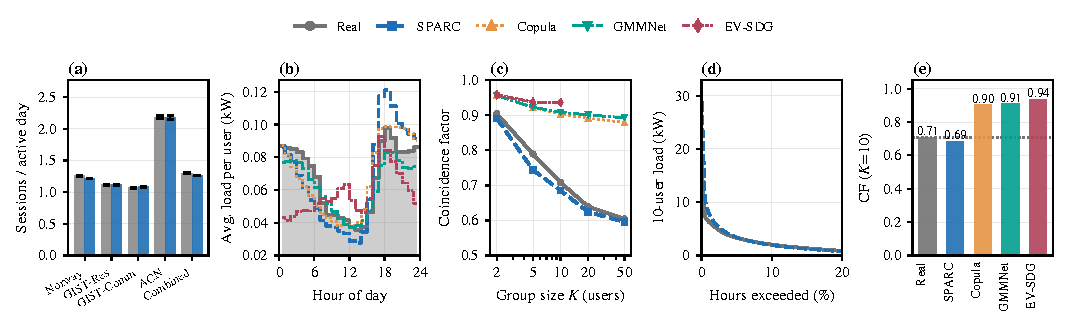
\includegraphics[width=\textwidth]{figures/fig_downstream_1x5_cfbar.pdf}
  \caption{(a)~Sessions per active day (mean$\pm$s.e.); on the combined pool: (b)~average weekday load per user; (c)~coincidence factor vs.\ group size $K$ (count-matched pseudo-users for baselines); (d)~$10$-user load-duration, real vs.\ SPARC; (e)~CF at $K=10$ (dotted: real).}
  \label{fig:downstream}
\end{figure*}

\subsection{Benchmark Against Baselines}
\label{subsec:benchmark}
We benchmark SPARC against three generators spanning the copula, deep-generative, and parametric families, along two axes: aggregate marginal fidelity, and the per-user and joint structure aggregate marginals cannot see. Every method is fit on the same cleaned sessions per dataset and emits a matched session count. SPARC statistics pool five seeds; baseline variability is over $100$ bootstrap resamples for the marginals and $30$ random pseudo-user partitions for the heterogeneity.

\emph{Copula~\cite{einolander2021}} (Einolander--Lahdelma): empirical marginals coupled by a multivariate Student-$t$ copula and drawn i.i.d.\ from the pooled joint: within-session dependence, but no user identity or session timing. \emph{GMMNet~\cite{li2024synthesis}}: conditional Gaussian-mixture density networks over the $(A,D,E)$ joint, Gibbs-sampled ($150$ epochs per dataset), reproducing marginals and cross-variable dependence but pooling all users and drawing sessions independently. \emph{EV-SDG~\cite{lahariya2020}}: a widely cited parametric generator (DBSCAN session clustering, per-cluster mixtures, and an inter-arrival-time process) with its generative horizon capped at $24$~h.

\emph{Why no per-user baseline?} No published session generator fits identifiable individuals. The closest family is cluster-based (Table~\ref{tab:litreview}): SPEECh~\cite{powell2022} and Van~Kriekinge~et~al.~\cite{vankriekinge2023} model $K \ll U$ behavioral types, so identity is lost within each cluster. The natural hierarchical alternative, one pooled generator fitted per user, fails at real sample sizes: deep generators need thousands of sessions per fit (P5), while the median user here has $138$ (Section~\ref{subsec:lowdata}). We therefore give the pooled baselines the strongest per-user evaluation an identity-free generator admits, count-matched pseudo-users (Table~\ref{tab:heterogeneity}, Fig.~\ref{fig:downstream}); the heterogeneity collapse and CF overestimate that follow are properties of the pooled class, not of a weak implementation.

Table~\ref{tab:benchmark} reports the aggregate marginals. The copula reproduces the pooled densities almost exactly ($\mathrm{KL}\le0.001$~nats on the large Norway and Combined pools), and SPARC is a close second throughout, even leading on arrival for the sparser GIST cohorts. GMMNet trails by a factor of three to ten, and EV-SDG degrades sharply on duration and energy: its $24$~h cap cannot represent Norway's overnight sessions, inflating the duration divergence to $17.9$~nats. Judged on marginals alone, one might simply prefer the copula.

Table~\ref{tab:heterogeneity} reverses that conclusion. We define $\sigma_A$ and $\sigma_D$ as the across-user standard deviation of each user's circular-mean arrival hour and mean plug-in duration, the direct signature of per-user heterogeneity~(P1). SPARC recovers the real spread within seed variation on every dataset (Norway $\sigma_D=5.46\pm0.13$ vs.\ real $5.66$); the pooled baselines collapse it three- to six-fold, since an exchangeable session bag makes every average user near-identical. The same separation appears in the $24$~h load shape, where SPARC is lowest on all five datasets.

Together the tables resolve the apparent copula advantage: a generator can be marginally exact yet manufacture a fleet of identical users, misrepresenting the diversity that governs coincident demand and transformer sizing. SPARC alone matches the marginals, the per-user heterogeneity~(P1), and the load shape, from tens of sessions per user~(P5) without per-context tuning~(P6).



\subsection{Downstream Operational Validity}
\label{subsec:downstream}

Fig.~\ref{fig:downstream}(b)--(e) evaluates whether the generated sessions support the grid studies of Section~\ref{sec:introduction}, with session power $E/D$ spread over each session. In panel~(b), SPARC is the only generator that tracks the full daily shape (morning decline, midday valley, evening ramp), though it overstates the evening peak, a consequence of the not-yet-modeled duration--energy dependence (Remark~\ref{rem:which-dependence}). Panels~(c) and~(e) report the coincidence factor $\mathrm{CF}(K) = \max_t \sum_{u \in K} \ell_u(t) / \sum_u \max_t \ell_u(t)$, the diversity metric behind transformer sizing. SPARC follows the real curve within $0.01$--$0.05$ at every group size, while the pooled baselines stay near $0.9$: their statistically identical users overstate coincidence by $28$--$48\%$ at $K = 10$, the collapse predicted in Section~\ref{sec:introduction}, oversizing transformer capacity accordingly. In panel~(d), the $10$-user pocket load-duration curves overlap through the operating range, with SPARC conservative only in the top $0.5\%$ of hours. Preserving per-user structure is thus what makes a synthetic fleet usable for sizing and coincidence studies.

\begin{table}[t]
\centering
\caption{Sparse-data sensitivity: fit on each driver's first $n$ sessions, evaluated against the \emph{full} history (KL, nats; median per-user error).}
\label{tab:lowdata}
\setlength{\tabcolsep}{4pt}
\footnotesize
\begin{tabular}{rcccccc}
\toprule
$n$ & $\mathrm{KL}_A$ & $\mathrm{KL}_D$ & $\mathrm{KL}_E$ & $\mathrm{MAE}_D$ (h) & $\mathrm{MAE}_E$ (kWh) & $\mathrm{MAE}_A$ (h) \\
\midrule
$10$  & 0.022 & 0.153 & 0.054 & 4.86 & 5.63 & 1.80 \\
$20$  & 0.014 & 0.103 & 0.025 & 2.93 & 3.45 & 1.16 \\
$30$  & 0.017 & 0.073 & 0.016 & 1.67 & 1.78 & 0.82 \\
$50$  & 0.015 & 0.053 & 0.020 & 1.55 & 1.37 & 0.52 \\
$100$ & 0.013 & 0.039 & 0.014 & 0.51 & 0.66 & 0.35 \\
\bottomrule
\end{tabular}
\end{table}

\subsection{Low-Data Sensitivity}
\label{subsec:lowdata}

P5 claims stable fits from tens of sessions per user; we now quantify it. SPARC is refit on the pooled driver cohorts ($155$ users) with each history truncated to its chronologically first $n \in \{10, 20, 30, 50, 100\}$ sessions, relaxing the inclusion rule accordingly, and every fit is evaluated against the user's \emph{full} record. A prefix preserves genuine consecutive pairs, mimicking a shorter collection campaign. Table~\ref{tab:lowdata} shows graceful degradation: every population KL stays within the L4 tolerance $\epsilon = 0.15$ down to $n = 20$, and at $n = 10$ only duration touches it ($0.153$); per-user error shrinks monotonically with history length ($4.9 \to 0.5$~h in mean duration). Fits are already usable at $20$--$30$ sessions, so the framework's history requirement is conservative rather than necessary.

\section{Conclusion}
\label{sec:conclusion}
We presented SPARC, a per-user semi-Markov paradigm that represents EV charging as each user's recurring session patterns. It pairs a session-as-state encoding with BIC-selected non-exponential per-bin marginals, a three-level fallback for sparse profiles, and a convolution diagnostic that couples duration and idle gap only where independence fails. Across four cohorts from three open datasets, both driver- and station-level, and their combined pool, every profile validates through the four-level protocol without per-context tuning; against copula, deep-generative, and parametric baselines, SPARC matches aggregate marginal fidelity while uniquely preserving the between-user heterogeneity pooled models discard. Future work includes seasonal factorization, charging-power time series, richer dependence via vine copulas, and anonymous public charging.

\bibliographystyle{IEEEtran}
\bibliography{myRef}

\end{document}
